% 图 8.24 锰氧化物 Ruddlesden-Popper 相 n=1/2/∞：MnO6 八面体片与 (La,Sr)-O 岩盐层交替
\documentclass[tikz,border=5pt]{standalone}
\usetikzlibrary{arrows.meta}
\usepackage{amsmath}
\usepackage{bm}
\usepackage{fontspec}
\setmainfont{Times New Roman}
\begin{document}
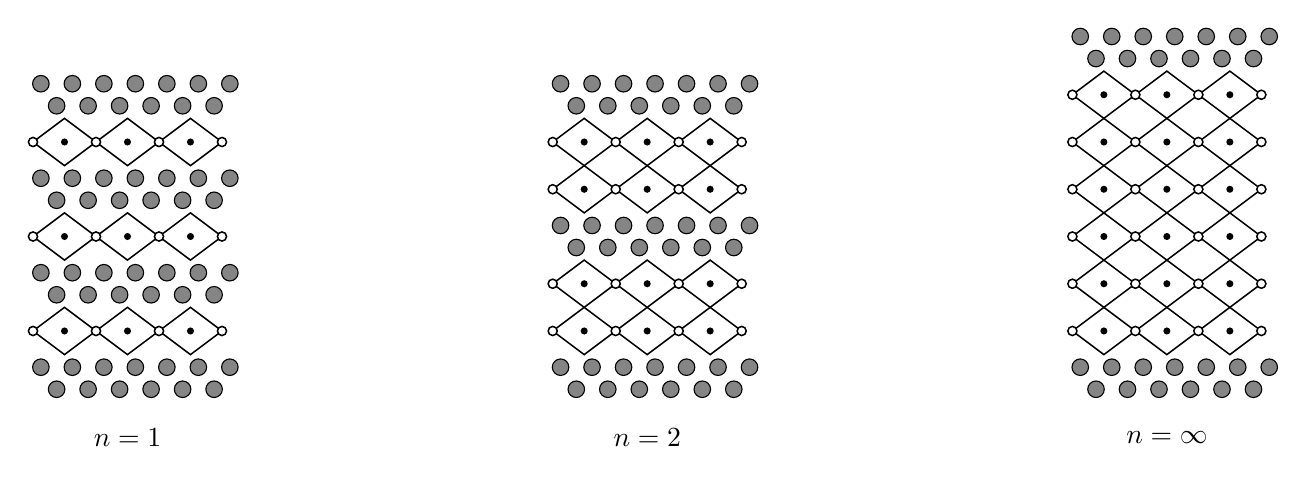
\begin{tikzpicture}[line width=0.8pt,>=Stealth]
% ---------- one row of three corner-sharing MnO6 octahedra (diamonds) ----------
% #1 = x origin, #2 = row height
\newcommand{\octrow}[2]{%
  \foreach \k in {0,1,2}{%
    \pgfmathsetmacro{\cx}{#1+0.4+\k*0.8}%
    \draw[line width=0.55] (\cx-0.4,#2) -- (\cx,{#2+0.3}) -- (\cx+0.4,#2) -- (\cx,{#2-0.3}) -- cycle;
  }
  \foreach \k in {0,1,2}{% Mn at body centres
    \pgfmathsetmacro{\cx}{#1+0.4+\k*0.8}%
    \fill (\cx,#2) circle (0.045);
  }
  \foreach \k in {0,...,3}{% O at shared vertices
    \pgfmathsetmacro{\vx}{#1+\k*0.8}%
    \draw[fill=white,line width=0.55] (\vx,#2) circle (0.058);
  }
}
% ---------- rock-salt (La,Sr)-O layer: two staggered rows of large cations ----------
% #1 = x origin, #2 = layer centre height
\newcommand{\rsrow}[2]{%
  \foreach \k in {0,...,6}{%
    \pgfmathsetmacro{\bx}{#1+0.1+\k*0.4}%
    \draw[fill=black!48,line width=0.4] (\bx,{#2+0.14}) circle (0.105);
  }
  \foreach \k in {0,...,5}{%
    \pgfmathsetmacro{\bx}{#1+0.3+\k*0.4}%
    \draw[fill=black!48,line width=0.4] (\bx,{#2-0.14}) circle (0.105);
  }
}
% ---------- n = 1 : single octahedron sheets, rock-salt between every sheet ----------
\begin{scope}[shift={(0,0)}]
  \octrow{0}{0.9}  \rsrow{0}{0.3}
  \octrow{0}{2.1}  \rsrow{0}{1.5}
  \octrow{0}{3.3}  \rsrow{0}{2.7}
                   \rsrow{0}{3.9}
  \node at (1.2,-0.45) {$n=1$};
\end{scope}
% ---------- n = 2 : double octahedron sheets, rock-salt between blocks ----------
\begin{scope}[shift={(3.3,0)}]
  \octrow{3.3}{0.9} \octrow{3.3}{1.5}   \rsrow{3.3}{0.3}
  \octrow{3.3}{2.7} \octrow{3.3}{3.3}   \rsrow{3.3}{2.1}
                                        \rsrow{3.3}{3.9}
  \node at (4.5,-0.45) {$n=2$};
\end{scope}
% ---------- n = infinity : continuous perovskite stack ----------
\begin{scope}[shift={(6.6,0)}]
  \octrow{6.6}{0.9} \octrow{6.6}{1.5} \octrow{6.6}{2.1}
  \octrow{6.6}{2.7} \octrow{6.6}{3.3} \octrow{6.6}{3.9}
  \rsrow{6.6}{0.3}  \rsrow{6.6}{4.5}
  \node at (7.8,-0.45) {$n=\infty$};
\end{scope}
\end{tikzpicture}
\end{document}
